\usepackage[margin=2cm]{geometry}

\begin{document}

\hypertarget{ejercicio-monitorizaciuxf3n-con-grafanaprometheus}{%
\section{Ejercicio Monitorización con
Grafana+Prometheus}\label{ejercicio-monitorizaciuxf3n-con-grafanaprometheus}}

\hypertarget{indicaciones}{%
\subsection{Indicaciones}\label{indicaciones}}

Se han hecho capturas de pantalla de todo el proceso y están adjuntas en
una carpeta aparte (\texttt{images}). Durante el documento se
referenciaran en qué imagenes aparecen las instrucciones que se usan. Se
ha hecho así para facilitar la lectura y poder consultar cualquier duda
en las imágenes. Se han indicado con (img\_) donde '\_' representa el
número de imagen (ese será su nombre en el directorio recién
mencionado). Se han adjuntado directamente además las que se piden de
forma directa en los ejercicios.

\hypertarget{monitorizaciuxf3n-de-servidor-linux}{%
\subsection{Monitorización de Servidor
Linux}\label{monitorizaciuxf3n-de-servidor-linux}}

\hypertarget{enunciado}{%
\subsubsection{Enunciado}\label{enunciado}}

Emplear la plataforma Prometheus + Grafana instalada para monitorizar
las prestaciones de un servidor Rocky corriendo en una VM. El alumno/a
puede elegir los componentes de Prometheus y Grafana que prefiera o
crear nuevos componentes por si mismo/a. No obstante, se sugiere emplear
como base el exporter de Linux para Prometheus, configurado como un
servicio y emplear como base algún dashboard predefinido para Grafana.
Siga las instrucciones de cada dashboard para posibles ajustes en
Prometheus. En Granafa vaya a \texttt{Dashboards\ →\ Import} y
proporcionar el \texttt{Id} del dashboard.

El dashboard debe recibir como identificador, el nombre y apellidos del
alumno/a en CamelCase junto con el sufijo ``Linux''. Por ejemplo,
mariaGarciaPerezLinux. Todos los paneles creados se presentarán con un
título que contenga las iniciales del alumno/a. Siguiendo con el ejemplo
anterior: \%CPU (MGP).

El alumno/a debe extender el dashboard anterior para incorporar
indicadores sobre el el nivel de activación (``Activo''/''Inactivo'',
1/0) de los servicios: SSHD y Apache Httpd en el equipo Linux
monitorizado.

Además, deberá agregar un nuevo panel sobre el nivel de uso total de la
CPU en tanto por ciento (\%). A este panel se le asociará una alarma
para que se dispare cuando la media del uso de CPU supere el 75\% de CPU
durante 5 minutos. Ponga de manifiesto el funcionamiento de la alarma
empleando alguna herramienta de carga de las vistas en clase (por
ejemplo, \texttt{stress}).

Para poner de manifiesto el funcionamiento de la monitorización, se
adjuntará una memoria en la que se presenten: - Descripción de la
secuencia de pasos realizada para ejecutar el exporter de Linux. Con
capturas de pantalla de los pasos seguidos para su ejecución y/o
configuración. - Capturas de pantalla de los monitores de Sshd y Httpd
poniendo de manifiesto su comportamiento cuando los servicios están
activos e inactivos. Captura de pantalla del monitor de uso de CPU antes
y después de lanzar la carga de CPU. - Captura de pantalla del comando
empleado para disparar la carga de CPU. - Captura de pantalla que ponga
de manifiesto el disparo de la alarma asociada al monitor de CPU

\hypertarget{resoluciuxf3n}{%
\subsubsection{Resolución}\label{resoluciuxf3n}}

En primer lugar se ha instalado en la máquina virtual \texttt{wget} y se
ha clonado el repositorio de github (img1, img2):

\begin{Shaded}
\begin{Highlighting}[]
\FunctionTok{sudo}\NormalTok{ dnf install wget}
\FunctionTok{sudo}\NormalTok{ wget https://github.com/prometheus/node\_exporter/releases/download/v1.9.1/node\_exporter{-}1.9.1.linux{-}amd64.tar.gz}
\end{Highlighting}
\end{Shaded}

Una vez descargado el archivo
\texttt{node\_exporter-1.9.1.linux-amd64.tar.gz} se ha descargado
\texttt{tar} y se ha extraído el contenido del archivo con (img3, img4)

\begin{Shaded}
\begin{Highlighting}[]
\FunctionTok{sudo}\NormalTok{ dnf install tar}
\FunctionTok{tar} \AttributeTok{{-}xvf}\NormalTok{ node\_exporter{-}1.9.1.linux{-}amd64.tar.gz}
\end{Highlighting}
\end{Shaded}

Se ha creado a continuación un usuario nuevo sin terminal ni shell
(img5), se le ha dado la propiedad del archivo descomprimido
anteriormente (img6) y se ha cambiado el nombre del archivo a
\texttt{node\_exporter} (para facilitar su uso). Finalmente se le ha
dado permiso de ejecución (img7)

\begin{Shaded}
\begin{Highlighting}[]
\ExtensionTok{useradd} \AttributeTok{{-}{-}no{-}create{-}home} \AttributeTok{{-}{-}shell}\NormalTok{ /bin/false node\_exporter}
\FunctionTok{chown} \AttributeTok{{-}R}\NormalTok{ node\_exporter:node\_exporter /opt/node\_exporter{-}1.9.1.linux{-}amd64}
\FunctionTok{mv}\NormalTok{ /opt/node\_exporter{-}1.9.1.linux{-}amd64 /opt/node\_exporter}
\FunctionTok{chmod}\NormalTok{ u+x /opt/node\_exporter}
\end{Highlighting}
\end{Shaded}

Después se ha creado un servicio para el exporter y se ha añadido la
información necesaria para el funcionamiento (img8, img9)

\begin{Shaded}
\begin{Highlighting}[]
\FunctionTok{touch}\NormalTok{ /etc/systemd/system/node\_exporter.service}
\FunctionTok{vi}\NormalTok{ /etc/systemd/system/node\_exporter.service}
\end{Highlighting}
\end{Shaded}

En el archivo se ha añadido el siguiente contenido (img10):

\begin{Shaded}
\begin{Highlighting}[]
\ExtensionTok{[Unit]}
\VariableTok{Description}\OperatorTok{=}\NormalTok{Node }\ExtensionTok{Exporter}
\VariableTok{Wants}\OperatorTok{=}\NormalTok{network{-}online.target}
\VariableTok{After}\OperatorTok{=}\NormalTok{network{-}online.target}

\ExtensionTok{[Service]}
\VariableTok{User}\OperatorTok{=}\NormalTok{node\_exporter}
\VariableTok{Group}\OperatorTok{=}\NormalTok{node\_exporter}
\VariableTok{Typer}\OperatorTok{=}\NormalTok{simple}
\VariableTok{ExecStart}\OperatorTok{=}\NormalTok{/opt/node\_exporter/node\_exporter}

\ExtensionTok{[Install]}
\VariableTok{WantedBy}\OperatorTok{=}\NormalTok{default.target}
\end{Highlighting}
\end{Shaded}

Una vez hecho esto se han recargado los demonios y se ha habilitado el
nuevo servicio recién creado (img11)

\begin{verbatim}
systemctl daemon-reexec
systemctl daemon-reload
systemctl enable node_exporter
\end{verbatim}

Se ha habilitado el puerto 9100 (img12)

\begin{Shaded}
\begin{Highlighting}[]
\ExtensionTok{firewall{-}cmd} \AttributeTok{{-}{-}permanent} \AttributeTok{{-}{-}add{-}port}\OperatorTok{=}\NormalTok{9100/tcp}
\ExtensionTok{firewall{-}cmd} \AttributeTok{{-}{-}reload}
\end{Highlighting}
\end{Shaded}

Para que el exporter pueda ver la nueva información que se quiere
recopilar se ha modificado una opción en su arranque. Para ello, en
lugar de modificar el servicio creado se han añadido directrices (un
parámetro para la ejecución). El proceso ha sido el siguiente (img13):

\begin{Shaded}
\begin{Highlighting}[]
\FunctionTok{sudo}\NormalTok{ mkdir }\AttributeTok{{-}p}\NormalTok{ /var/lib/node\_exporter/textfile\_collector}
\FunctionTok{sudo}\NormalTok{ systemctl edit node\_exporter}
\end{Highlighting}
\end{Shaded}

Con esta última instrucción se nos abre un archivo al que se le va
añadir la siguiente información (img14):

\begin{Shaded}
\begin{Highlighting}[]
\ExtensionTok{[Service]}
\VariableTok{ExecStart}\OperatorTok{=}
\VariableTok{ExecStart}\OperatorTok{=}\NormalTok{/usr/local/bin/node\_exporter }\ExtensionTok{{-}{-}collector.textfile.directory=/var/lib/node\_exporter/textfile\_collector}
\end{Highlighting}
\end{Shaded}

Se le ha dado la propiedad del \texttt{textfile\_collector} al
\texttt{node\_exporter} y se han recargado los demonios y el servicio
\texttt{node\_exporter} (img15):

\begin{Shaded}
\begin{Highlighting}[]
\FunctionTok{sudo}\NormalTok{ chown node\_exporter:node\_exporter /var/lib/node\_exporter/textfile\_collector}
\FunctionTok{sudo}\NormalTok{ systemctl daemon{-}reexec}
\FunctionTok{sudo}\NormalTok{ systemctl restart node\_exporter}
\end{Highlighting}
\end{Shaded}

Una vez hecho esto solo nos queda indicar qué parámetros queremos
exportar. Para ello se ha modificado el archivo (img16)

\begin{Shaded}
\begin{Highlighting}[]
\FunctionTok{sudo}\NormalTok{ vi /usr/local/bin/check\_services.sh}
\end{Highlighting}
\end{Shaded}

Y se ha añadido el siguiente contenido (img17):

\begin{Shaded}
\begin{Highlighting}[]
\CommentTok{\#!/bin/bash}

\VariableTok{OUTPUT\_FILE}\OperatorTok{=}\StringTok{"/var/lib/node\_exporter/textfile\_collector/service\_status.prom"}

\BuiltInTok{echo} \StringTok{"\# HELP service\_up Whether a systemd service is up (1) or down (0)"} \OperatorTok{\textgreater{}} \VariableTok{$OUTPUT\_FILE}
\BuiltInTok{echo} \StringTok{"\# TYPE service\_up gauge"} \OperatorTok{\textgreater{}\textgreater{}} \VariableTok{$OUTPUT\_FILE}

\ControlFlowTok{for}\NormalTok{ service }\KeywordTok{in}\NormalTok{ httpd sshd}\KeywordTok{;} \ControlFlowTok{do}
    \ControlFlowTok{if} \ExtensionTok{systemctl}\NormalTok{ is{-}active }\AttributeTok{{-}{-}quiet} \VariableTok{$service}\KeywordTok{;} \ControlFlowTok{then}
        \BuiltInTok{echo} \StringTok{"service\_up\{service=}\DataTypeTok{\textbackslash{}"}\VariableTok{$service}\DataTypeTok{\textbackslash{}"}\StringTok{\} 1"} \OperatorTok{\textgreater{}\textgreater{}} \VariableTok{$OUTPUT\_FILE}
    \ControlFlowTok{else} 
        \BuiltInTok{echo} \StringTok{"service\_up\{service=}\DataTypeTok{\textbackslash{}"}\VariableTok{$service}\DataTypeTok{\textbackslash{}"}\StringTok{\} 0"} \OperatorTok{\textgreater{}\textgreater{}} \VariableTok{$OUTPUT\_FILE}
    \ControlFlowTok{fi}
\ControlFlowTok{done}
\end{Highlighting}
\end{Shaded}

Después le daremos la propiedad al \texttt{node\_exporter} (img18) y
permiso de ejecución:

\begin{Shaded}
\begin{Highlighting}[]
\FunctionTok{sudo}\NormalTok{ chmod u+x /usr/local/bin/check\_services.sh}
\FunctionTok{sudo}\NormalTok{ chown node\_exporter:node\_exporter /var/lib/node\_exporter/textfile\_collector/service\_status.prom}
\end{Highlighting}
\end{Shaded}

Con este script mandamos al archivo \texttt{service\_status.prom} 4
líneas. Las 2 primeras son comentarios que ayudaran a otras tareas. Las
2 últimas serán de la forma:

\begin{verbatim}
service_up{service=httpd} *
service_up{service=httpd} *
\end{verbatim}

Donde en '*' aparecerá un número (0 o 1) que indica si el servicio entre
llaves está activo o no (es fácil de leer en el script).

Solo nos queda hacer que este script se ejecute periódicamente para
poder comprobar de forma continua el estado de estos servicios. Para
ello vamos a ejecutar los siguientes comandos (no tengo imagen de su
ejecución):

\begin{Shaded}
\begin{Highlighting}[]
\FunctionTok{sudo}\NormalTok{ crontab }\AttributeTok{{-}e}
\end{Highlighting}
\end{Shaded}

Y añadimos la siguiente línea al archivo:

\begin{verbatim}
* * * * * /usr/local/bin/check_services.sh
\end{verbatim}

Con esto hacemos que el script anterior se ejecute cada minuto. Una vez
hecho esto ya hemos finalizado la configuración en la máquina virtual
(el servidor que queremos monitorizar). Recargamos los demonios (img19)

\begin{Shaded}
\begin{Highlighting}[]
\ExtensionTok{systemctl}\NormalTok{ daemon{-}reload}
\ExtensionTok{systemctl}\NormalTok{ daemon{-}reexec}
\ExtensionTok{systemctl}\NormalTok{ restart node\_exporter}
\end{Highlighting}
\end{Shaded}

\begin{center}\rule{0.5\linewidth}{0.5pt}\end{center}

Una vez añadido el servicio de exporter de la máquina virtual se ha
lanzado el \texttt{docker} del host (sobre el directorio \texttt{progra}
creado de acuerdo a la documentación) (img20)

\begin{Shaded}
\begin{Highlighting}[]
\FunctionTok{sudo}\NormalTok{ docker compose up}
\end{Highlighting}
\end{Shaded}

Con esto ya tendremos disponible en el puerto 9090 Prometheus (img21) y
en el puerto 4000 Grafana en \texttt{localhost}. Configuramos el
\texttt{Data\ Source} en Grafana para que lea las métricas de
Prometheus.

En Frafana podemos importar un dashboard a partir de su id. En mi caso
he elegido el modelo con id \texttt{1860} (por ser bastante completo).

Ahora pasamos a añadir las dos nuevas métricas que nos pide el
ejercicio. Para ello se añade un nuevo panel y en el Query que se
despliega añadimos el siguiente código (img22):

\begin{verbatim}
service_up{service="sshd"}
\end{verbatim}

En las métricas de la derecha podemos cambiar el título del panel y
ponerle por ejemplo \texttt{SSHD\ Service\ {[}JMV{]}}. En Units podemos
ponerlo de tipo \texttt{Bool}, en concreto \texttt{On/Off} para mejorar
la visibilidad de la variable. Podemos también hacerlo de tipo
\texttt{Stat} (para no ver una gráfica lineal sino únicamente el valor)
y añadir thresolds para que se vea verde cuando esté activo y rojo
cuando esté inactivo (img23).

Si repetimos este proceso una vez más pero con el código

\begin{verbatim}
service_up{service="httpd"}
\end{verbatim}

podremos obtener una vista como la siguiente (img24):

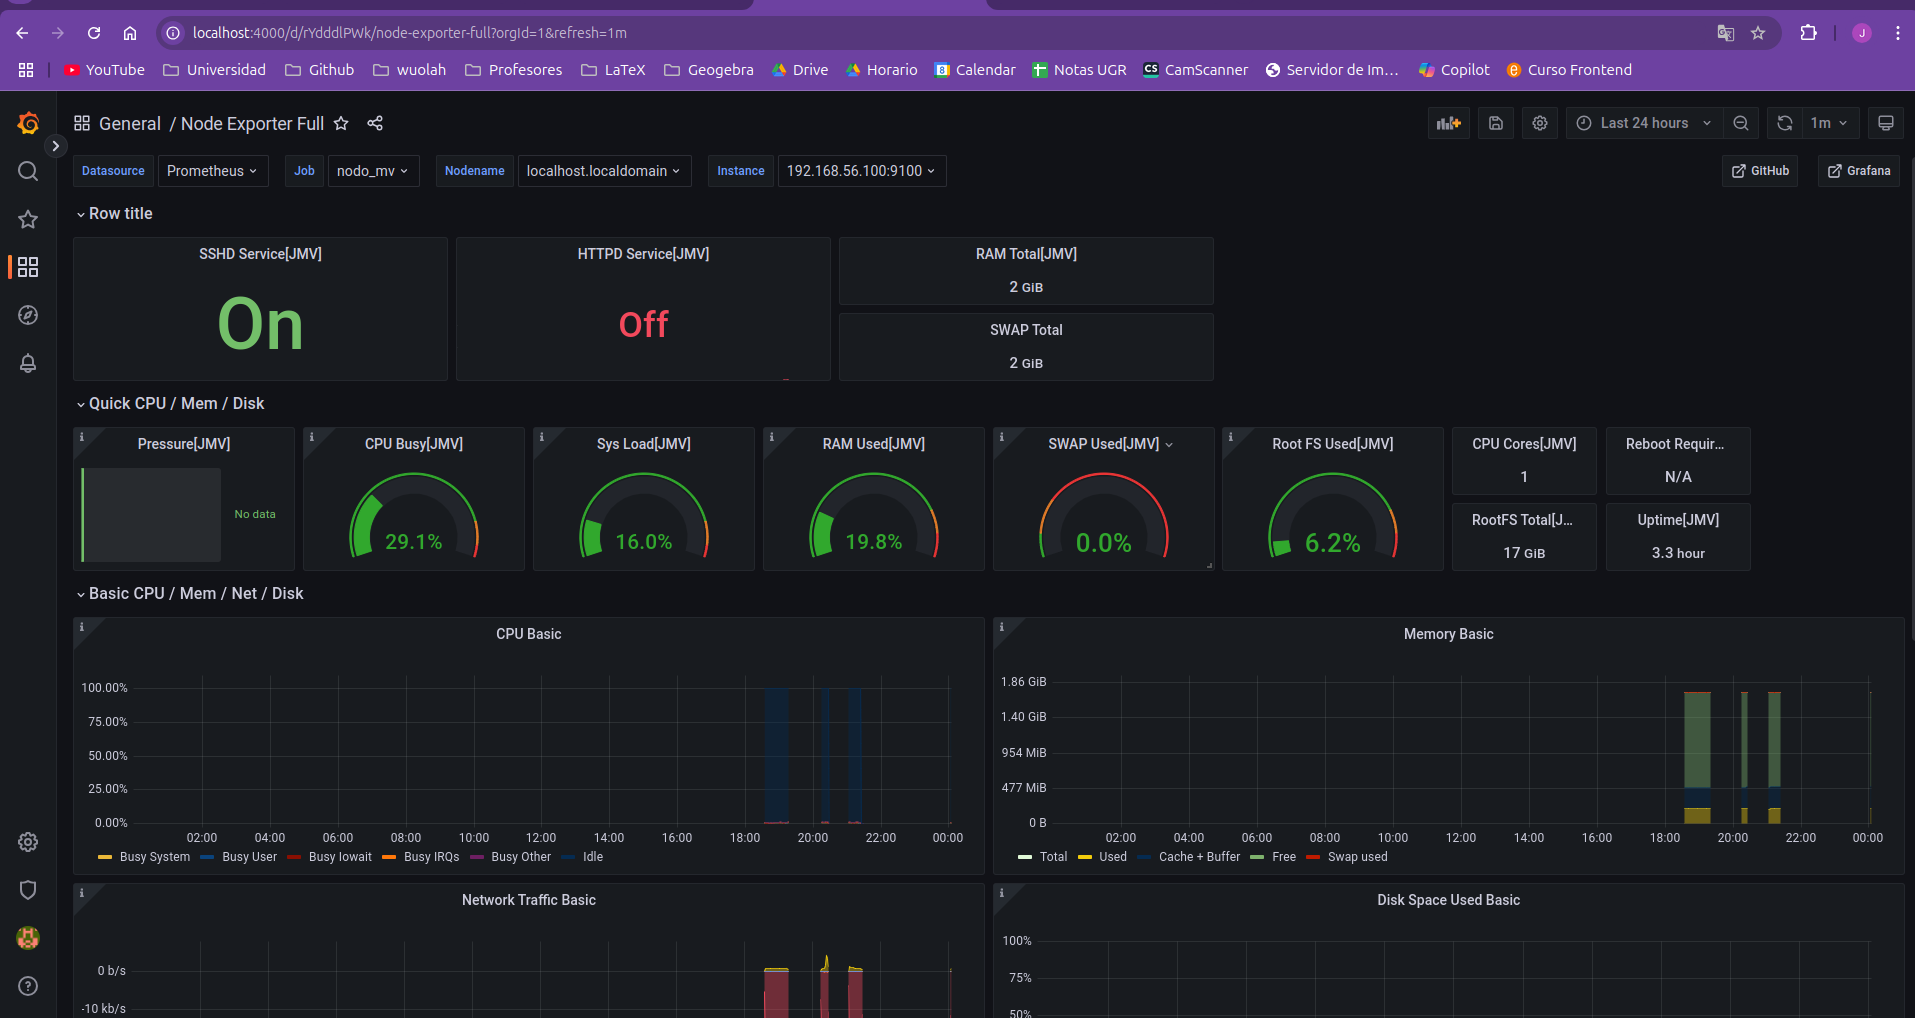
\includegraphics{./images_numeradas/img24.png}

Donde ya tenemos los paneles pedidos. Ahora podemos pasar a hacer
pruebas en los servidores para comprobar si funcionan correctamente
estos paneles.

Comenzamos instalando \texttt{httpd} en el servidor (img25):

\begin{Shaded}
\begin{Highlighting}[]
\FunctionTok{sudo}\NormalTok{ dnf install httpd}
\end{Highlighting}
\end{Shaded}

Podemos ver que inicialmente el panel \texttt{Httpd\ Service\ {[}JMV{]}}
se encuentra en estado \texttt{Off} (img26) :
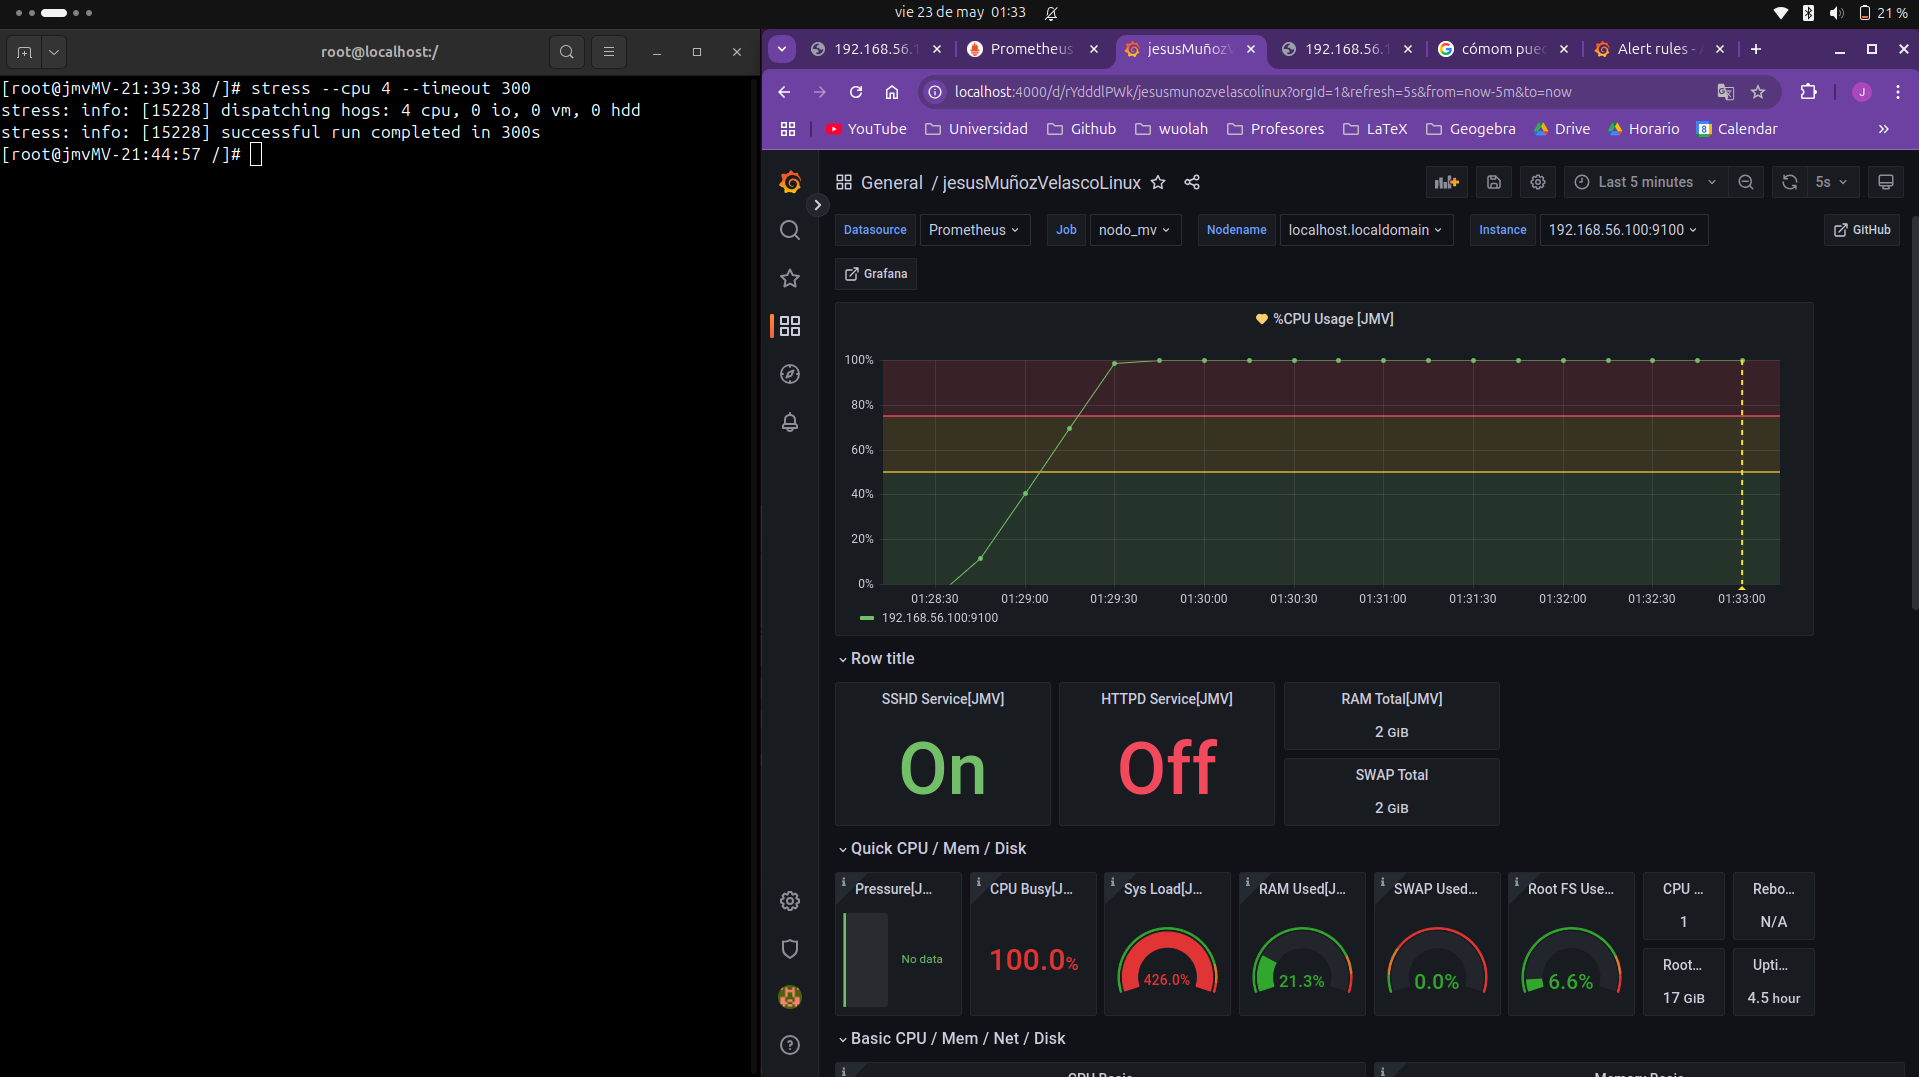
\includegraphics{./images_numeradas/img26.png}

Si ahora probamos a iniciar el servicio \texttt{httpd} obtenemos
(img27):

\begin{Shaded}
\begin{Highlighting}[]
\ExtensionTok{systemctl}\NormalTok{ start httpd}
\end{Highlighting}
\end{Shaded}

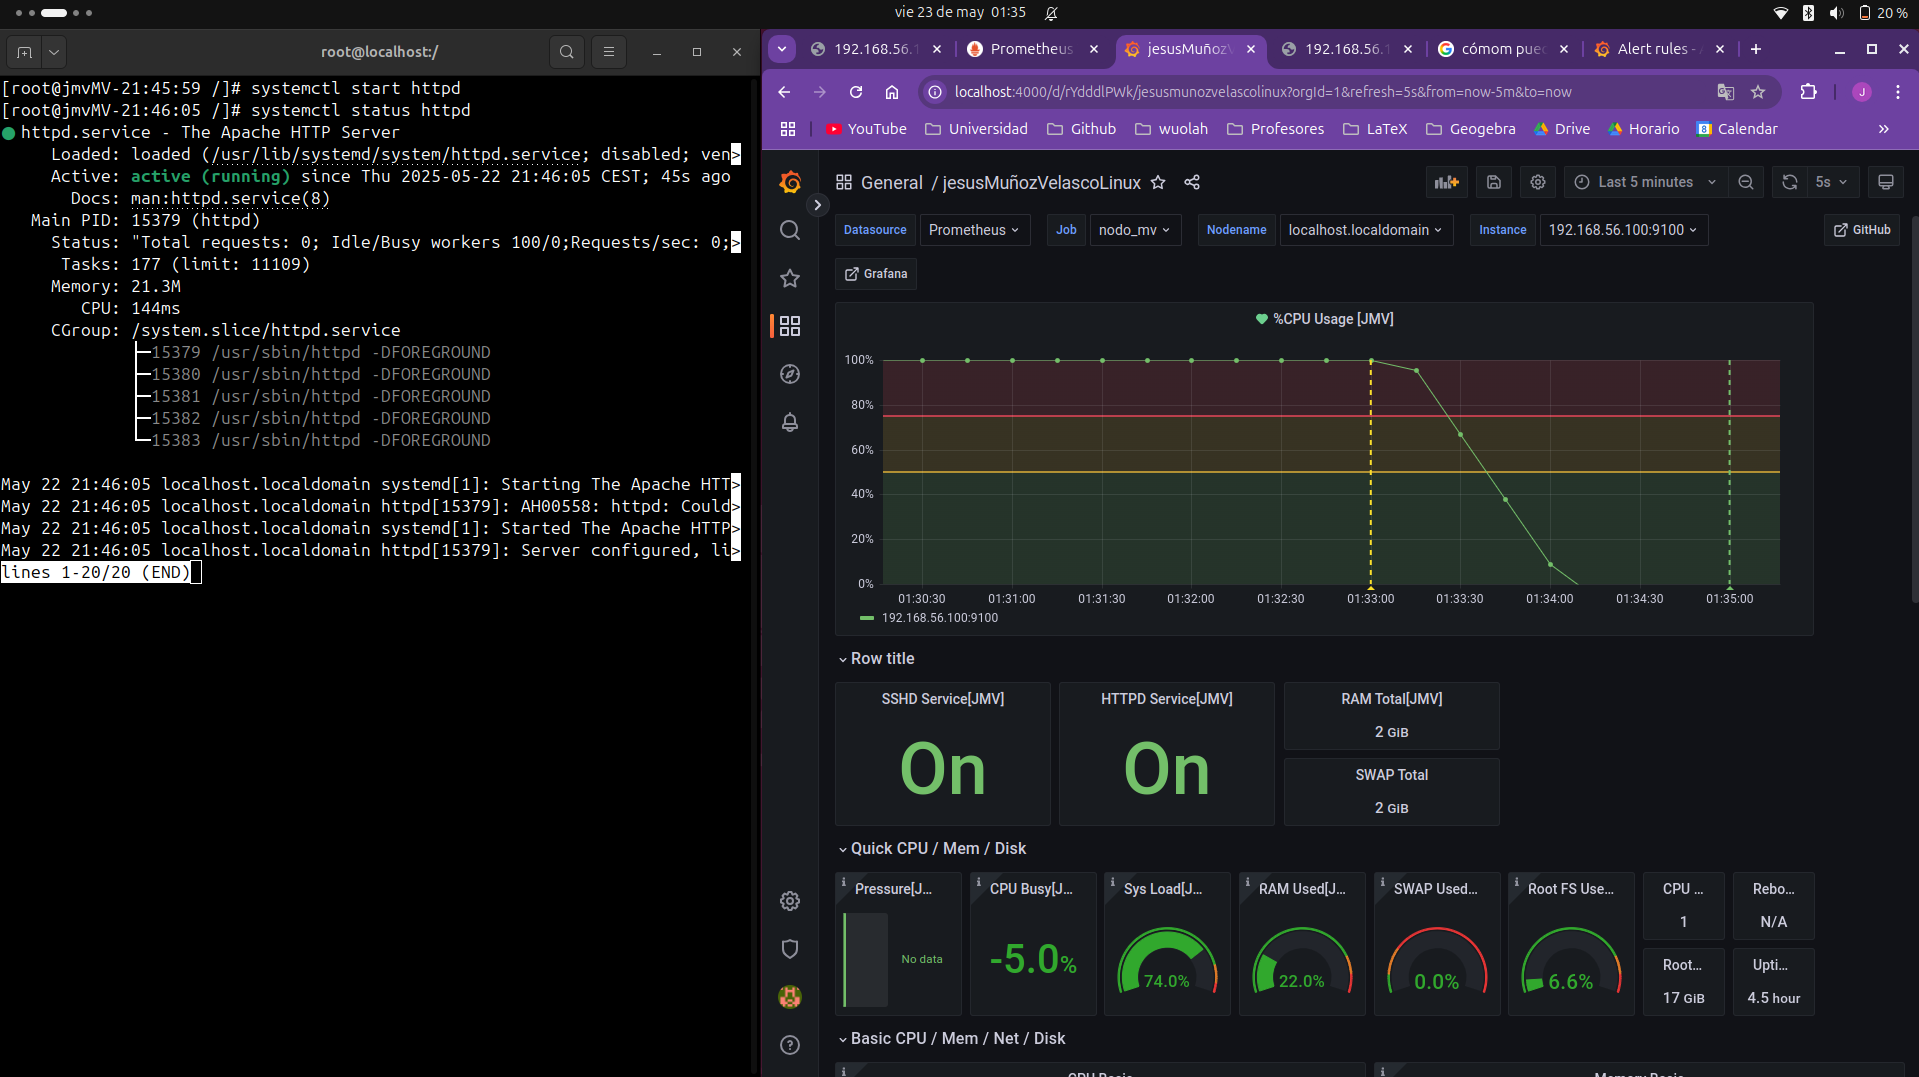
\includegraphics{./images_numeradas/img27.png}

Y vemos que efectivamente se activa el panel correspondiente.

Probamos ahora a desactivar el servicio \texttt{sshd} (img28):

\begin{Shaded}
\begin{Highlighting}[]
\ExtensionTok{systemctl}\NormalTok{ stop sshd}
\end{Highlighting}
\end{Shaded}

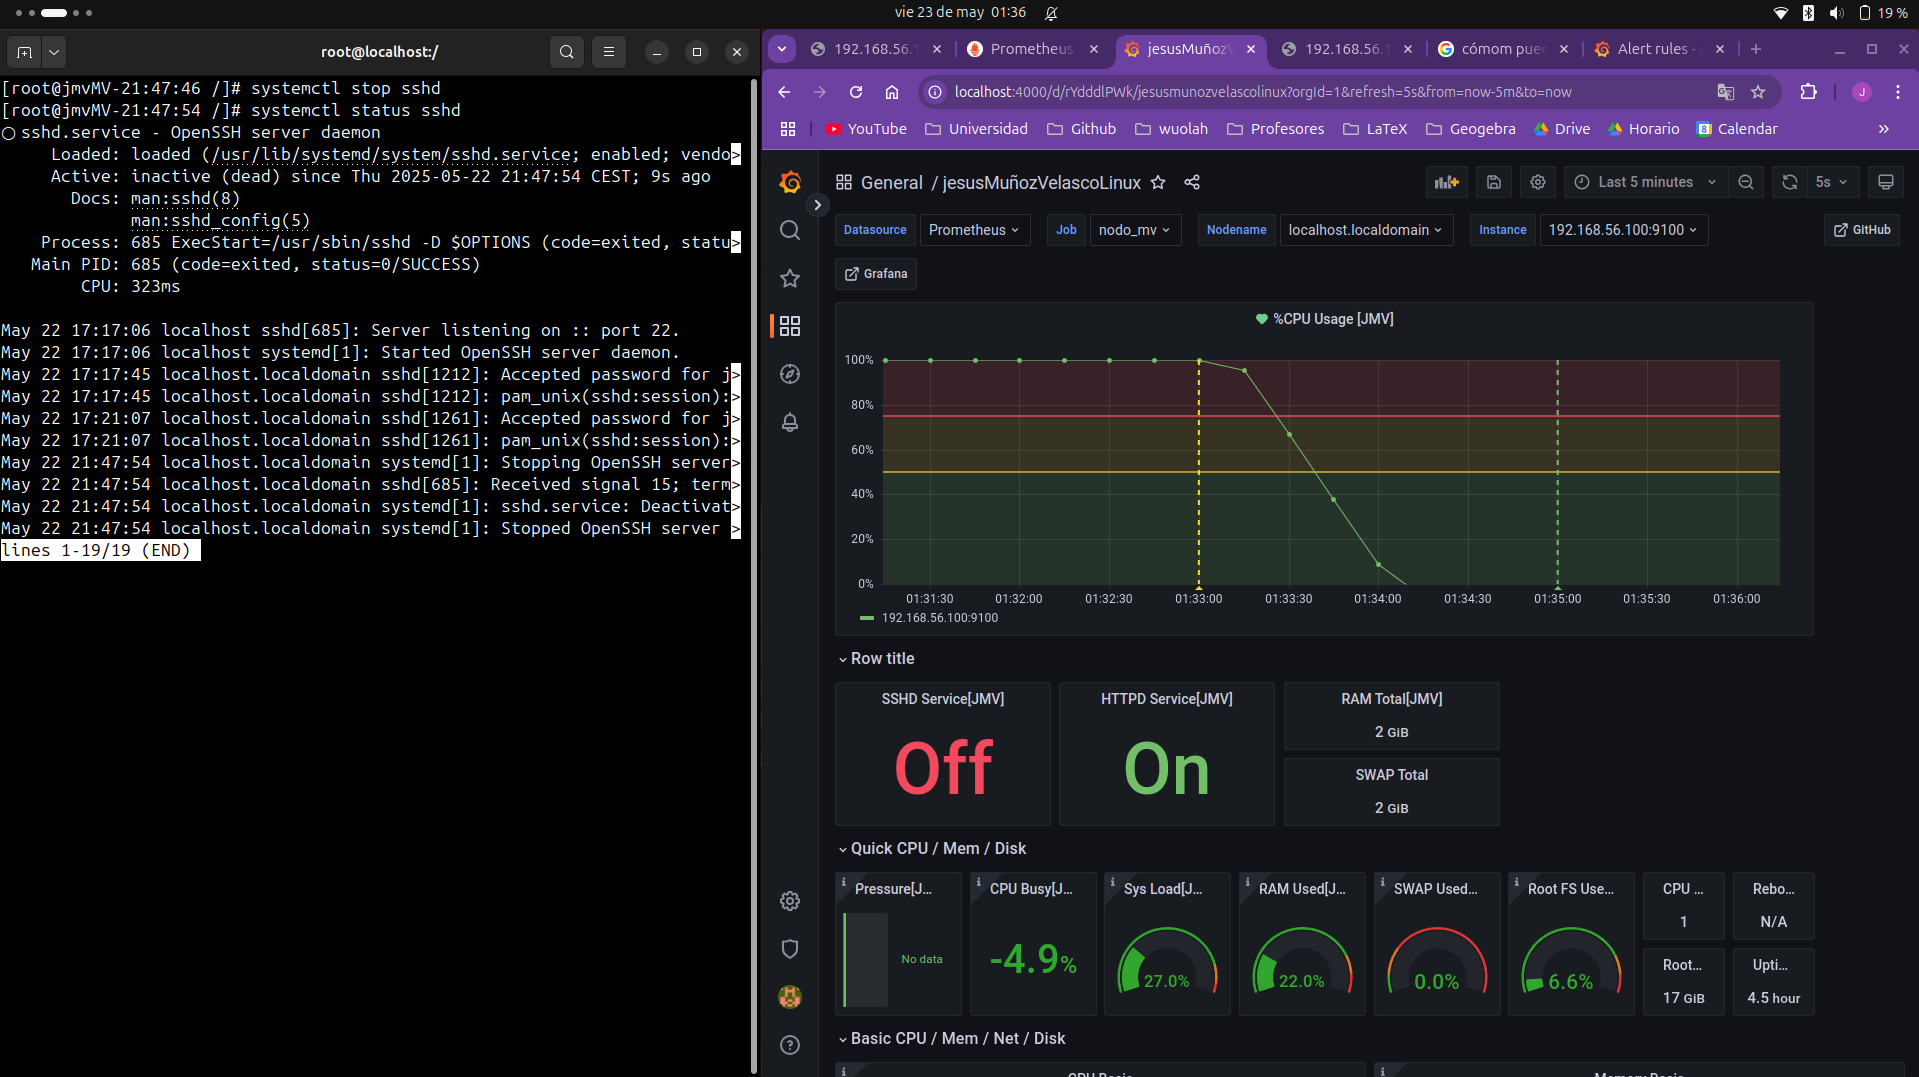
\includegraphics{./images_numeradas/img28.png}

Y vemos que efectivamente se desactiva. Probamos nuevamente a desactivar
también \texttt{httpd} (img29):

\begin{Shaded}
\begin{Highlighting}[]
\ExtensionTok{systemctl}\NormalTok{ stop httpd}
\end{Highlighting}
\end{Shaded}

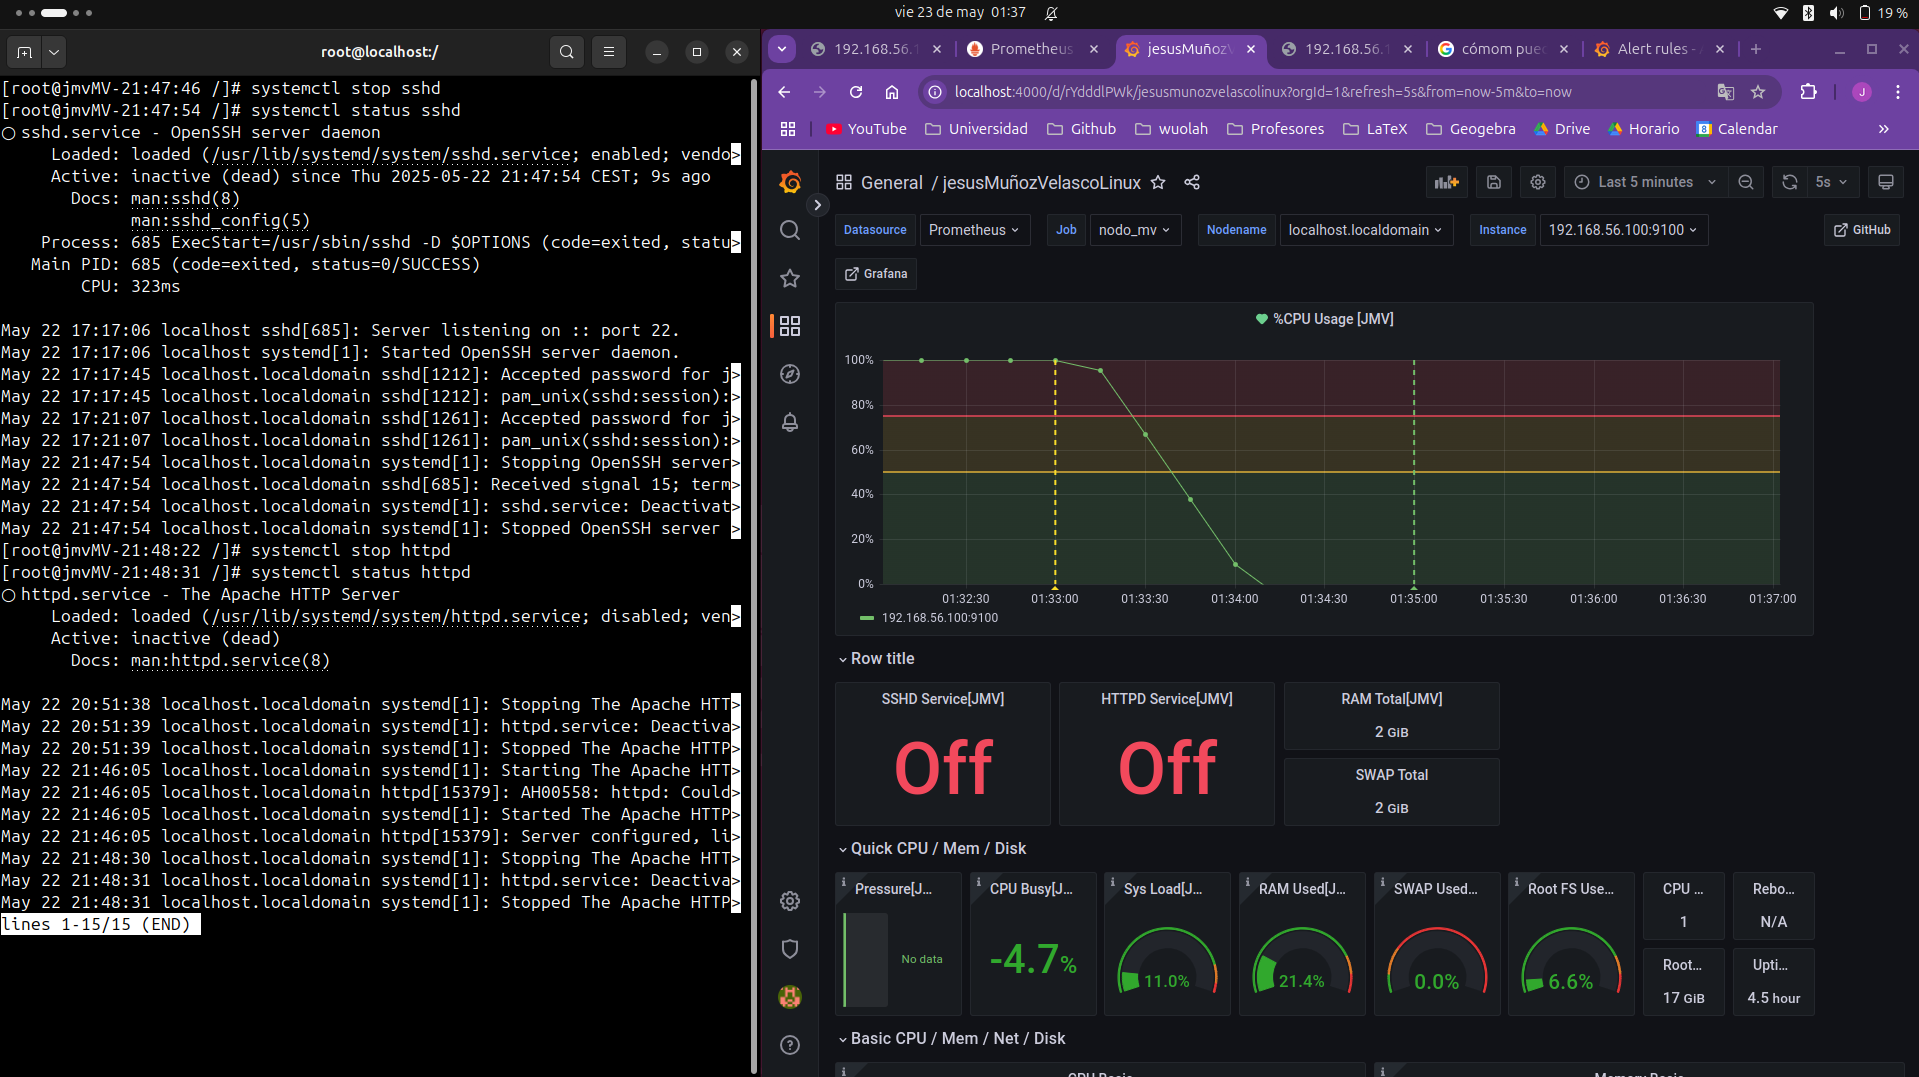
\includegraphics{./images_numeradas/img29.png}

Finalmente podemos activar los dos a la vez y tenemos el siguiente
resultado (img30):

\begin{Shaded}
\begin{Highlighting}[]
\ExtensionTok{systemctl}\NormalTok{ start httpd}
\ExtensionTok{systemctl}\NormalTok{ start sshd}
\end{Highlighting}
\end{Shaded}

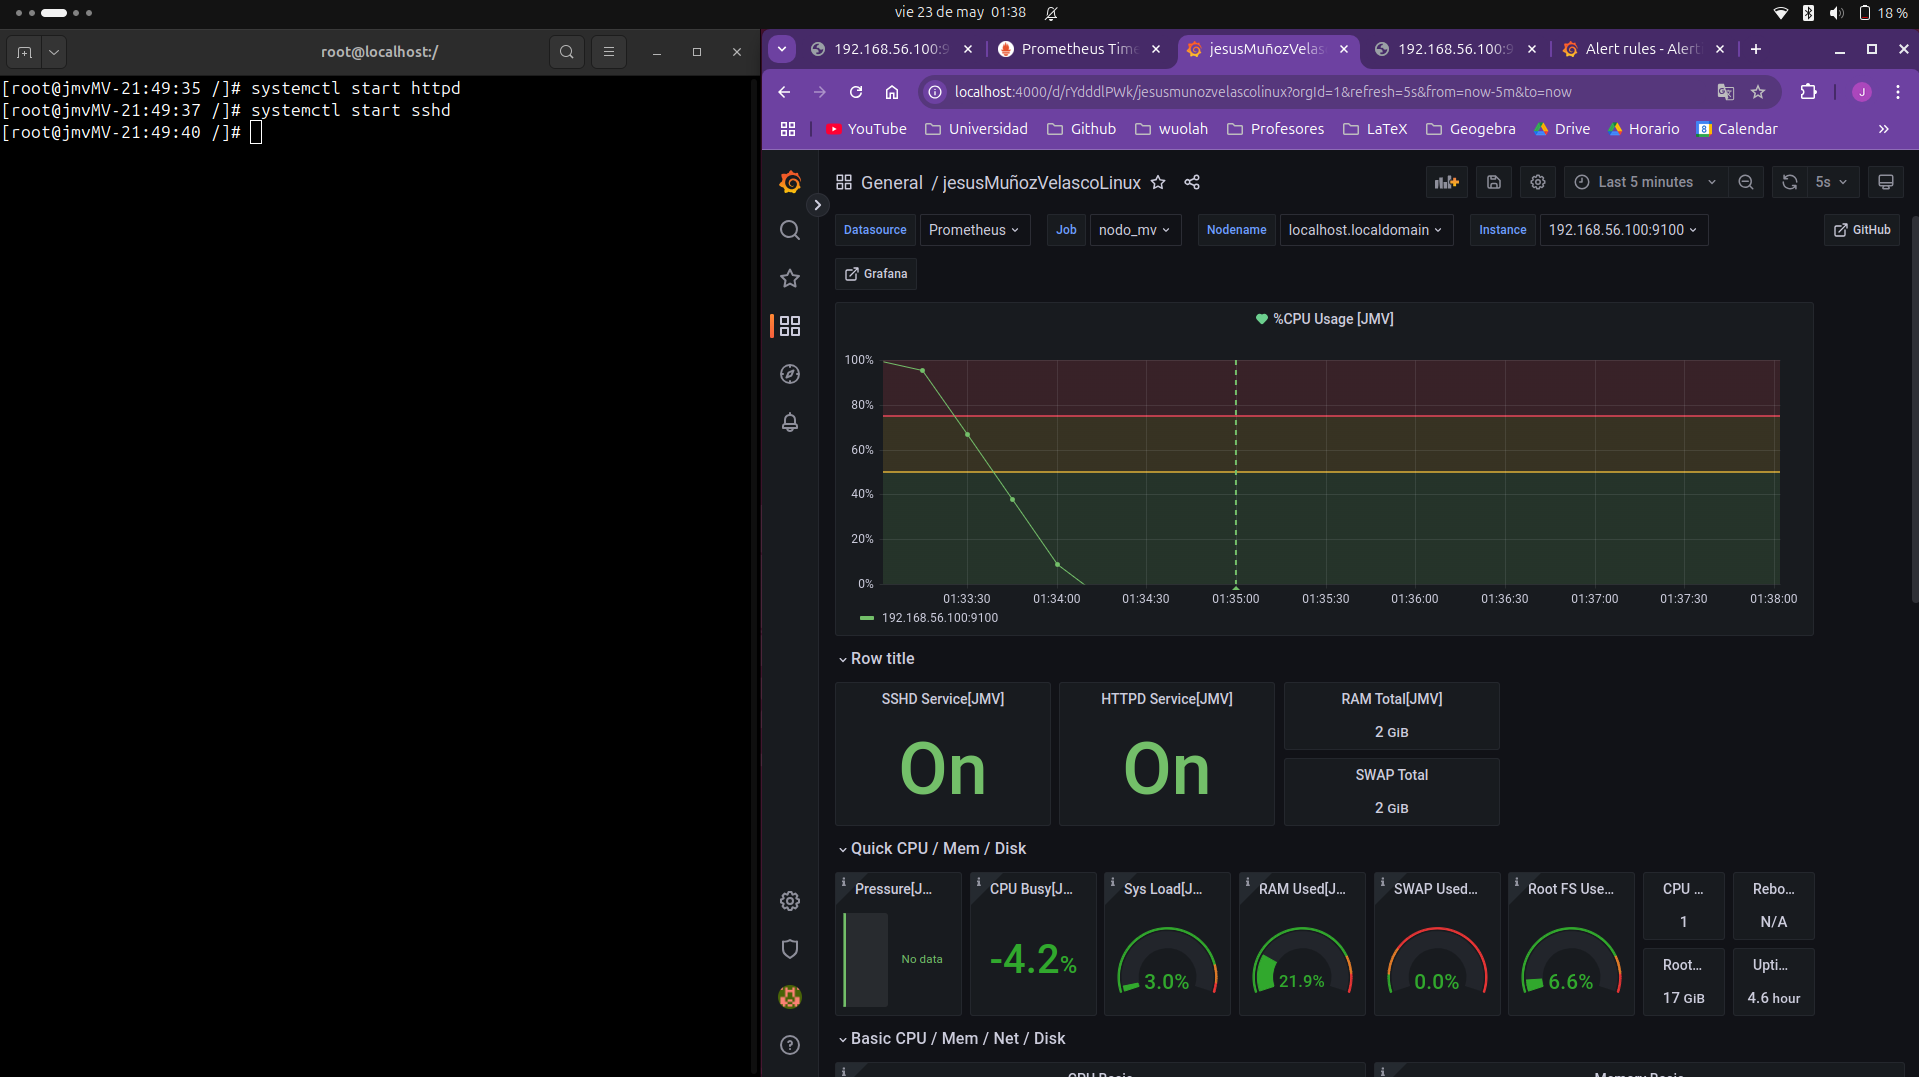
\includegraphics{./images_numeradas/img30.png}

Vamos ahora con el panel para medir el uso de la CPU. Creamos un nuevo
panel y añadimos el siguiente Query (img31):

\begin{verbatim}
100 - (avg by (instance) (rate(node_cpu_seconds_total{mode="idle"}[1m])) * 100)
\end{verbatim}

Podemos tocar los tresholds de nuevo para darle un aspecto más
atractivo. Finalizada la creación de este panel es hora de crear una
alerta. Le damos a alerts y añadimos una nueva alerta (img32).

Le indicamos la misma métrica que antes y en la expresión B añadimos
\texttt{WHEN\ last\ OF\ A\ IS\ ABOVE\ 75}. Una vez hecho esto terminamos
de configurar la alerta poniéndole \texttt{Evaluate\ 1m\ for\ 5m} para
que salte a los 5 min comprobándolo cada minuto. Podemos pasar ya a
probar el panel y la alerta (img33). Ejecutamos en la máquina virtual:

\begin{Shaded}
\begin{Highlighting}[]
\ExtensionTok{stress} \AttributeTok{{-}{-}cpu}\NormalTok{ 4 }\AttributeTok{{-}{-}timeout}\NormalTok{ 360}
\end{Highlighting}
\end{Shaded}

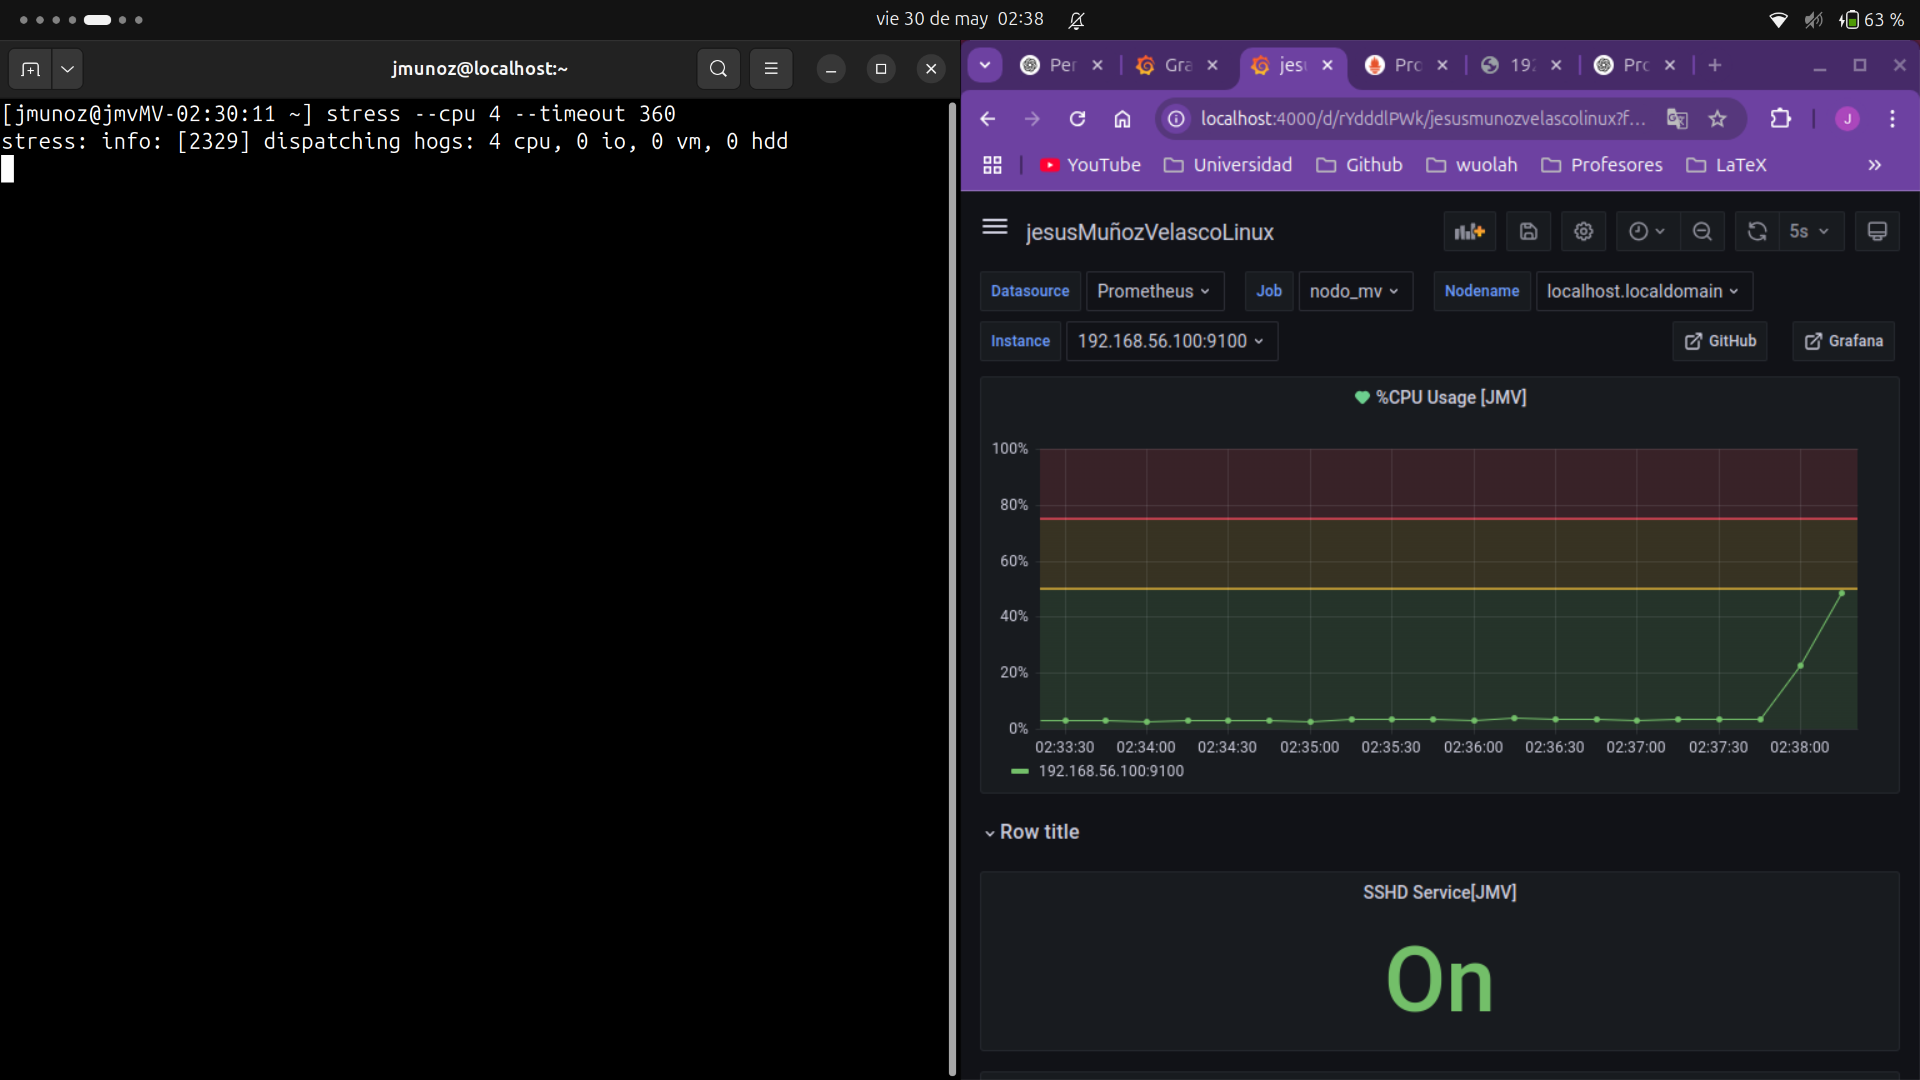
\includegraphics{./images_numeradas/img33.png}

Y vemos cómo empieza a subir el uso de la CPU en el panel recién creado.
Si vemos un poco más observamos que cuando supera el 75\% (línea roja)
se dispara la alarma pero en estado \texttt{pending} (img34):

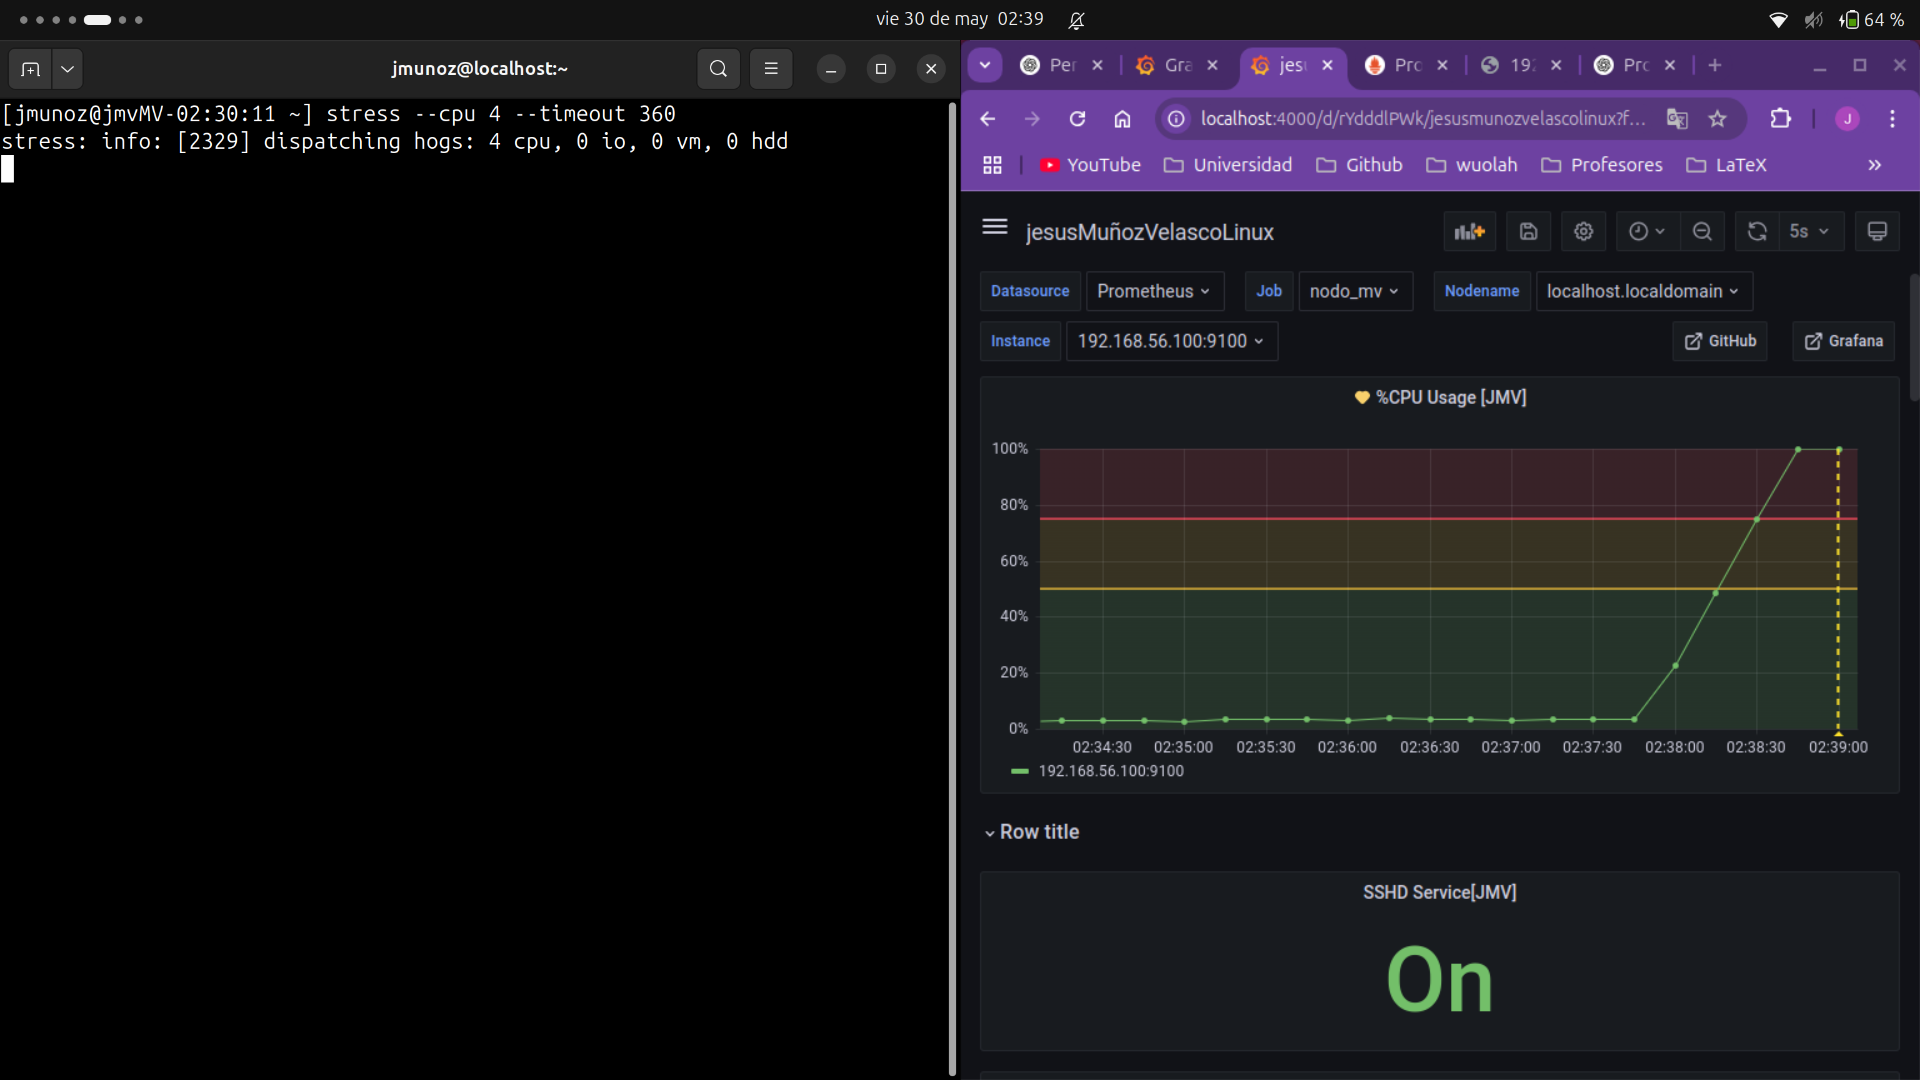
\includegraphics{./images_numeradas/img34.png}

Ahora empezará a contar 5 minutos hasta que se cumpla la condición para
que salte la alarma (img35):

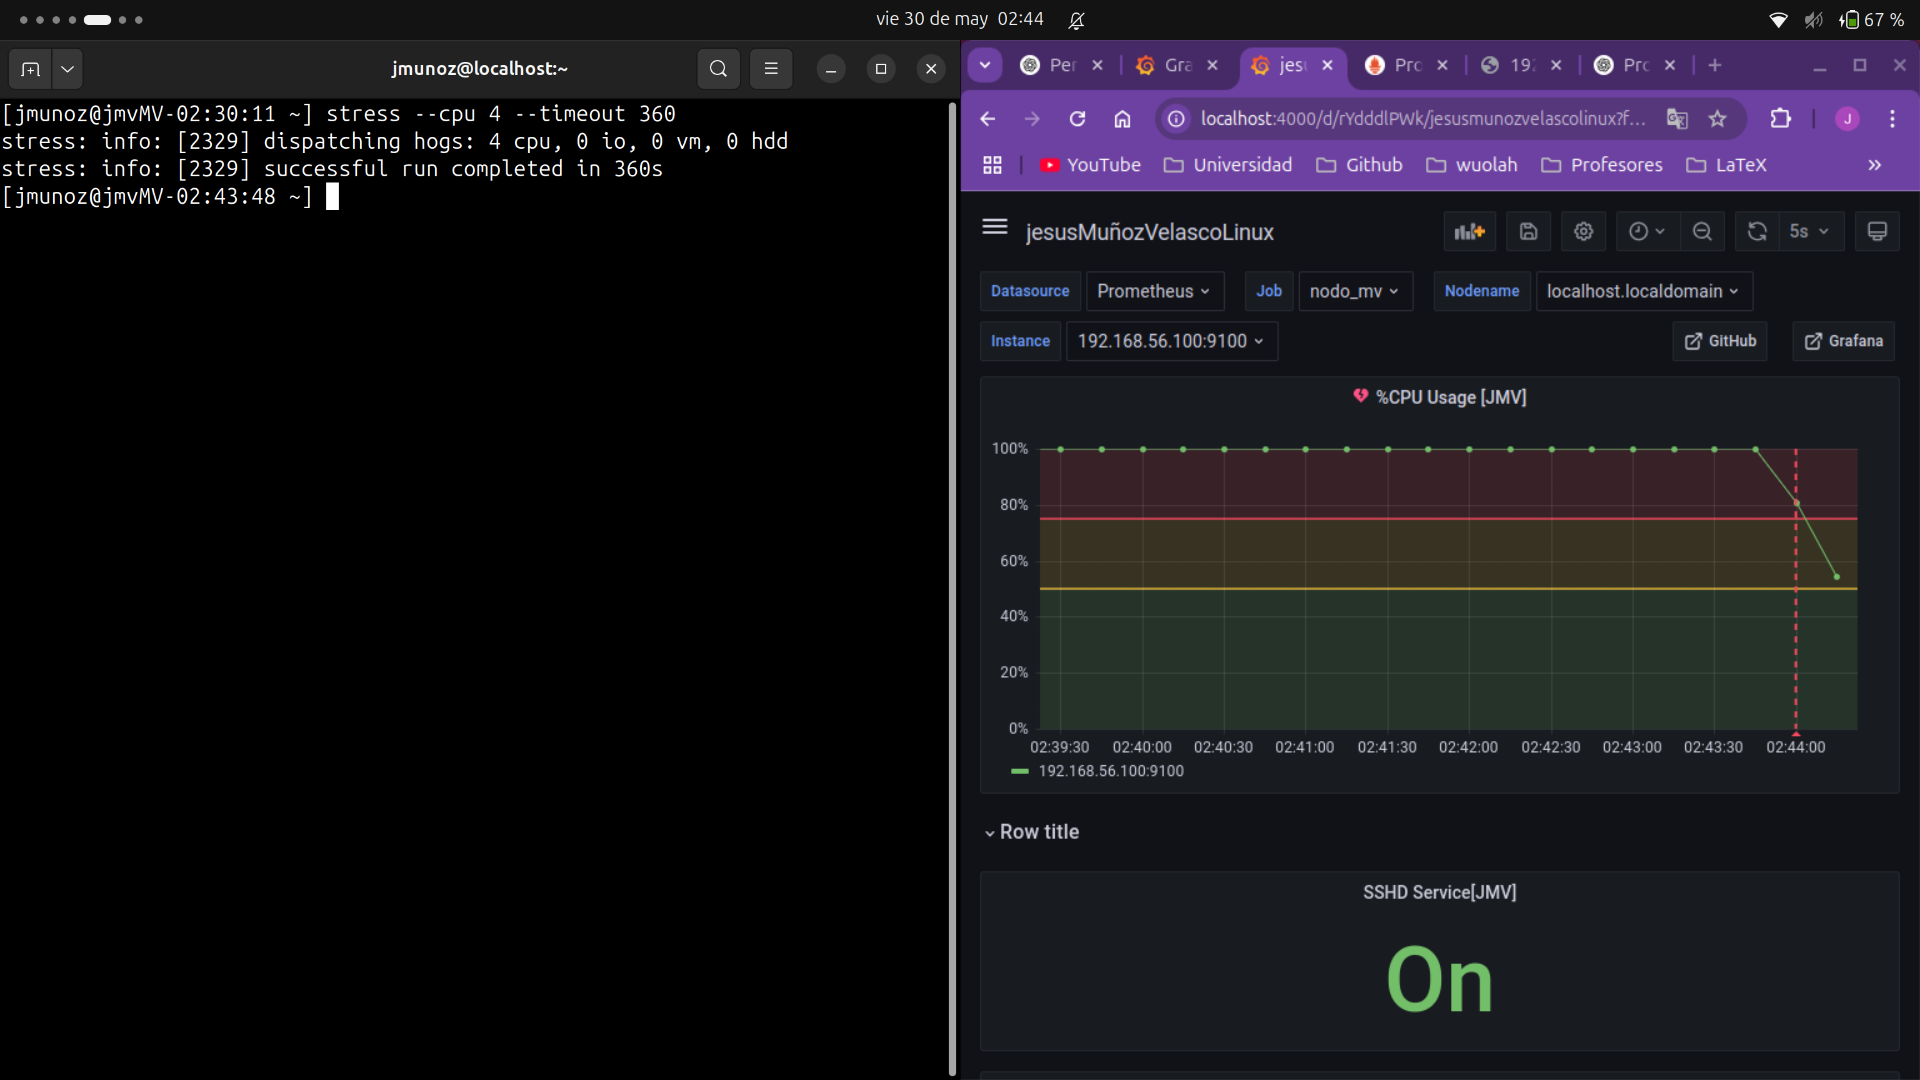
\includegraphics{./images_numeradas/img35.png}

Si lo dejamos un poco más vemos cómo de desactiva la alerta al volver a
un uso bajo de la CPU (img36):

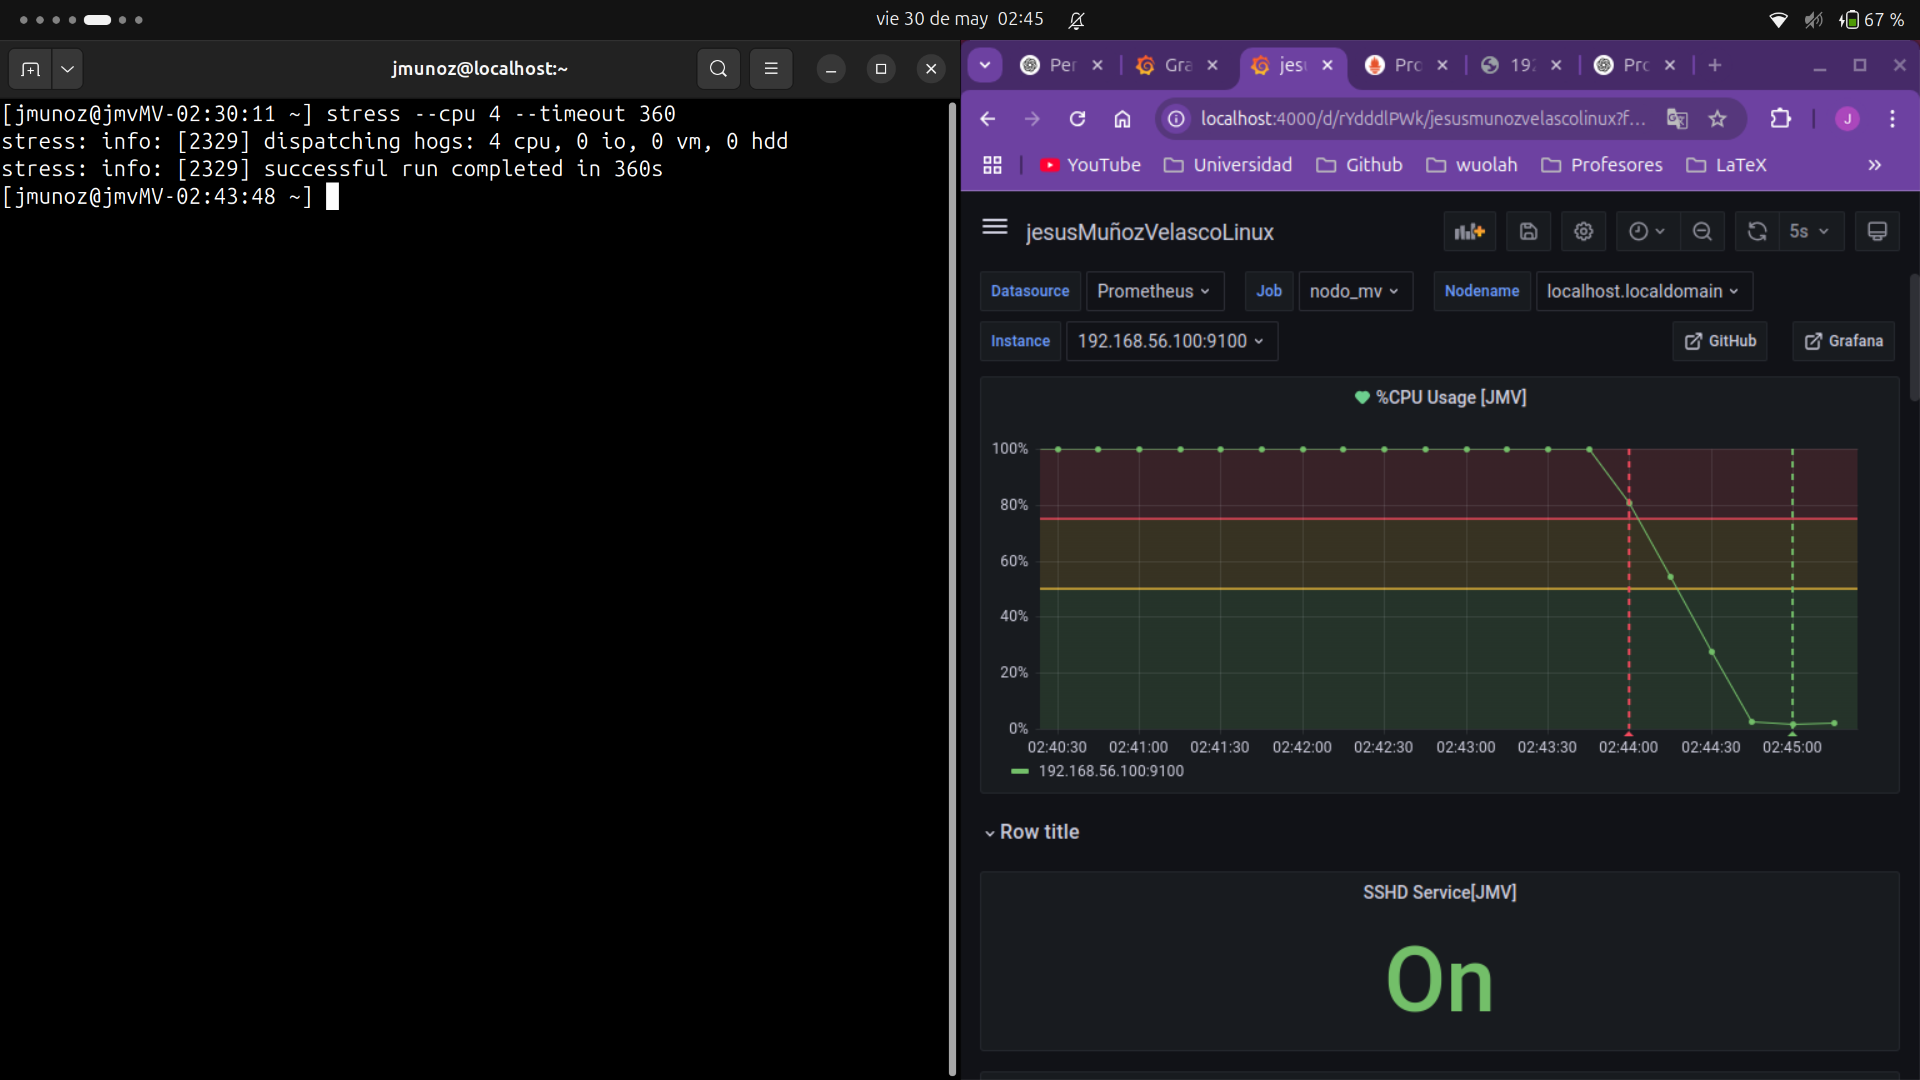
\includegraphics{./images_numeradas/img36.png}

\hypertarget{monitorizaciuxf3n-de-api-web}{%
\subsection{Monitorización de API
WEB}\label{monitorizaciuxf3n-de-api-web}}

\hypertarget{enunciado-1}{%
\subsubsection{Enunciado}\label{enunciado-1}}

La aplicación empleada en apartado anterior para la prueba de carga,
expone en el path ``/metrics'' los indicadores de NodeJS para
Prometheus. Para más información, el exporter de Prometheus de la API
Web se ha generado empleando los componentes estandar: prom-client y
express-prom-bundle.

Cree un nuevo Dashboard con algunas de las métricas expuestas. Para el
dashboard emplee como nombre su nombre y apellidos en CamelCase seguido
del sufijo API. Por ejemplo, anaTorrentRamonetAPI. Todos los paneles
creados se presentarán con un título que contenga las iniciales del
alumno/a. Siguiendo con el ejemplo anterior: \%Memoria (ATR).

Cree un monitores para las siguientes métricas: - Tiempos de respuesta
de los endpoints de la API (http\_request\_duration\_seconds\_bucket) -
Memoria disponible (nodejs\_heap\_size\_total\_bytes) vs la usada
actualmente (nodejs\_heap\_size\_used\_bytes) - Uso de CPU
(process\_cpu\_seconds\_total)

Realice una memoria de prácticas en la que se ponga de manifiesto la
ejecución de la prueba de carga diseñada para Jmeter y se aprecie el
efecto de la misma en los monitores anteriormente descritos.

\hypertarget{resoluciuxf3n-1}{%
\subsection{Resolución}\label{resoluciuxf3n-1}}

\end{document}
